\begin{frame}[noframenumbering,plain]
    \setcounter{framenumber}{1}
    \maketitle
\end{frame}

\begin{frame}
\frametitle{Обучение с подкреплением}
\begin{columns}
\column{0.4\linewidth}
  \centering
    \begin{tikzpicture}
            \node[anchor=south west,inner sep=0] (image) at (0,0) {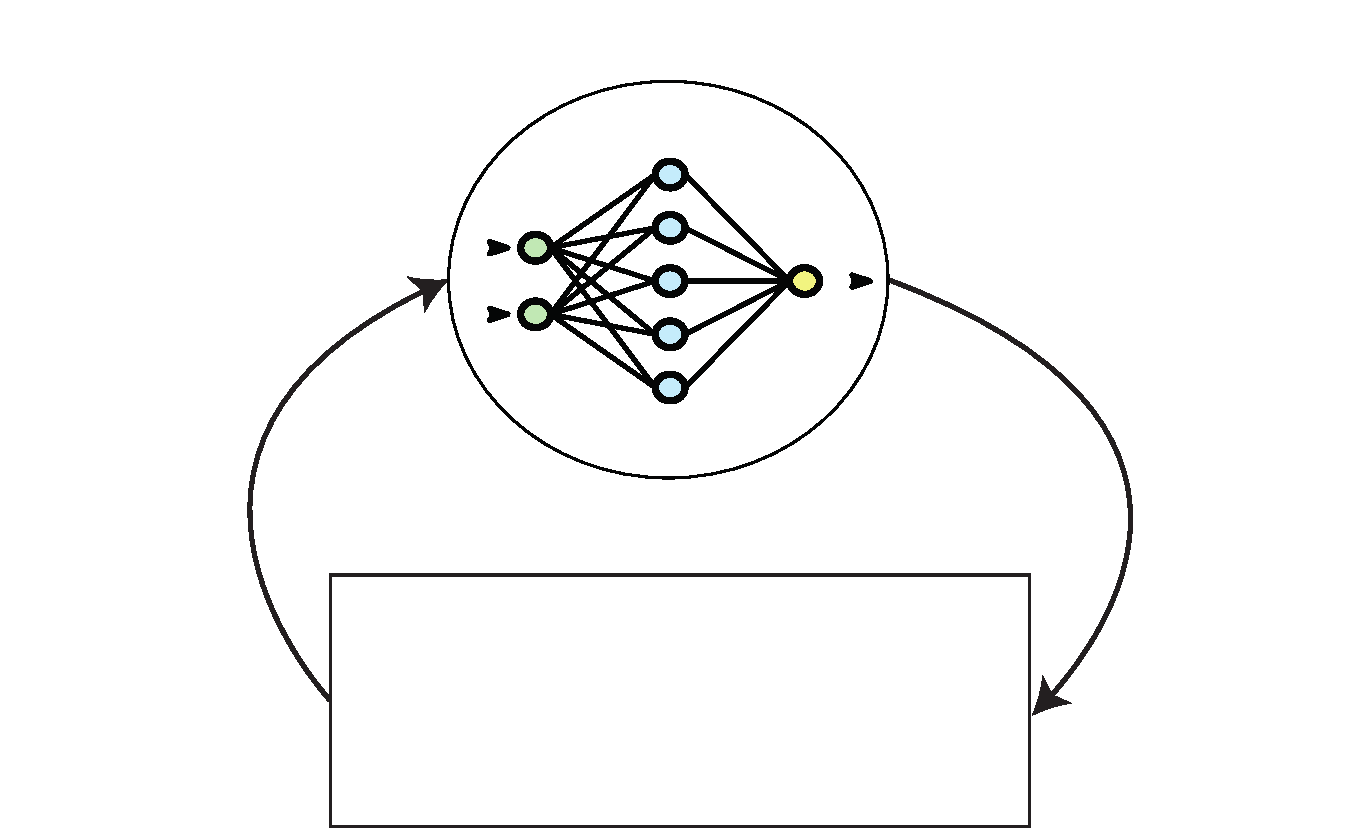
\includegraphics[width=1\linewidth]{Presentation/images/rl_setting_no_text.pdf}};
            \node[align=center,font={\small}] at (0.4,1) {s, r,\\done};
            \node[align=center,font={\small}] at (2.2,0.4) {среда};
            \node[align=center,font={\small}] at (2.1,2.6) {агент};
            \node[align=center,font={\small}] at (3.8,1) {a};
        \end{tikzpicture}
  %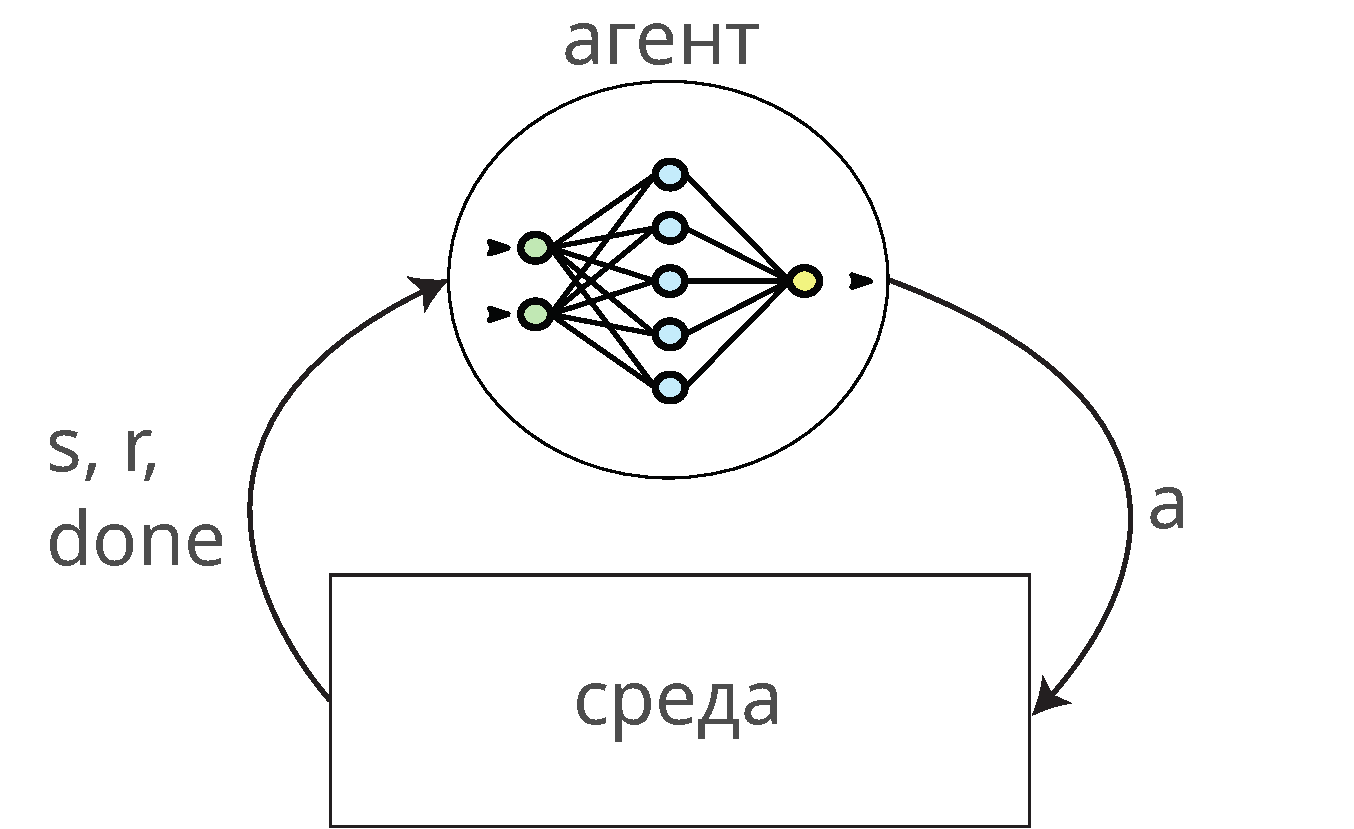
\includegraphics[width=1\linewidth]{Presentation/images/rl_setting_ru.pdf}
  \vspace{-10pt}
  \begin{equation*}
    <\mathcal{S, A, R, P}, \gamma>
  \end{equation*}

  \begin{align*}
  % & s_{t+1} \sim p(s_t, a) \\
  % & r_{t+1} = \mathcal{R}(s_t, a, s_{t+1}) \\
  % & \ex_{\tau \sim \pi} [G(\tau)] = \ex_{\tau \sim \pi} \left[r_0 + \gamma r_{1} + \gamma ^ 2 r_{2} + ...\right] \\
  & V^{\pi}(s_t) = \ex_{\tau \sim \pi}\left[\sum \gamma ^t r_{t}\right] \\
  & Q^{\pi}(s_t, a_t) = \ex_{\tau \sim \pi}\left[r_t + \sum \gamma ^{t + 1} r_{t + 1}\right] \\
  & \tau - \text{траектория}
  \end{align*}

\column{0.5\linewidth}
\centering
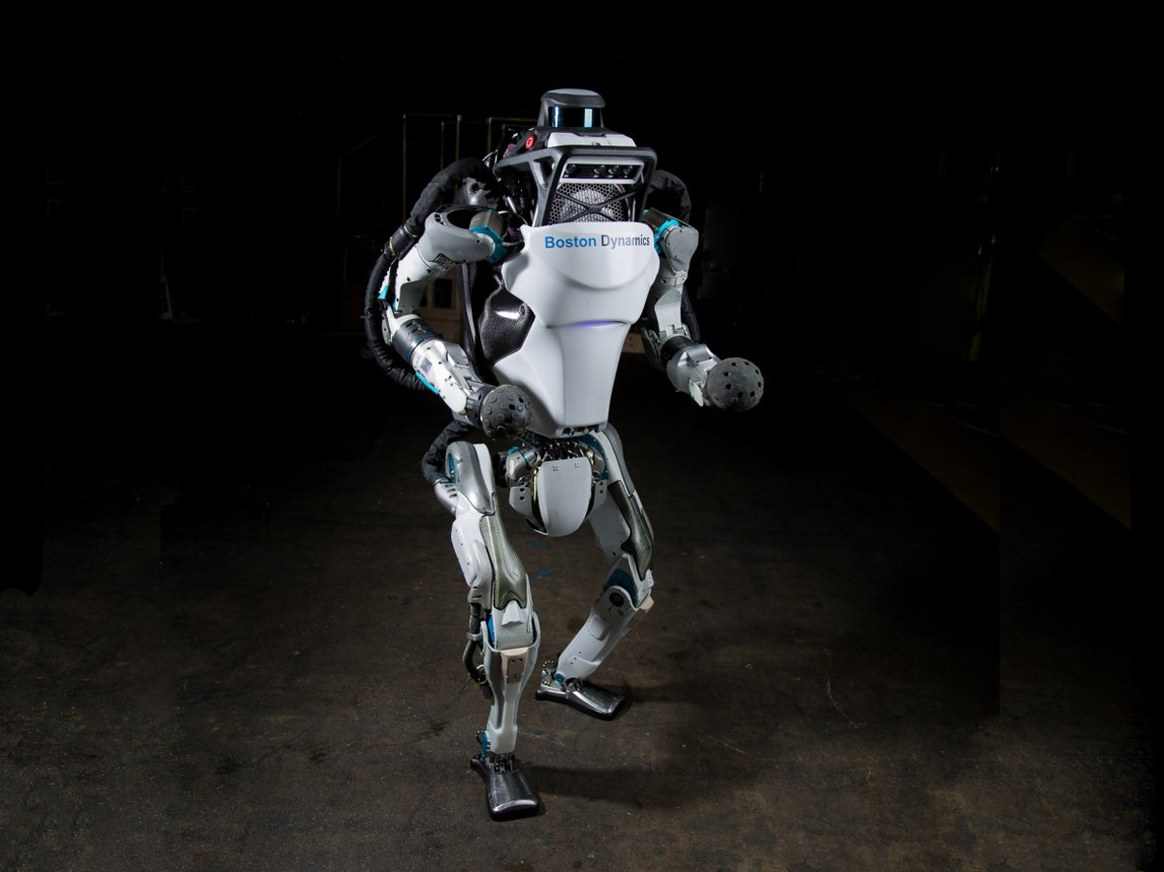
\includegraphics[width=0.8\linewidth]{Presentation/images/boston_dunamics.jpg}

\vspace{10pt}
\centering
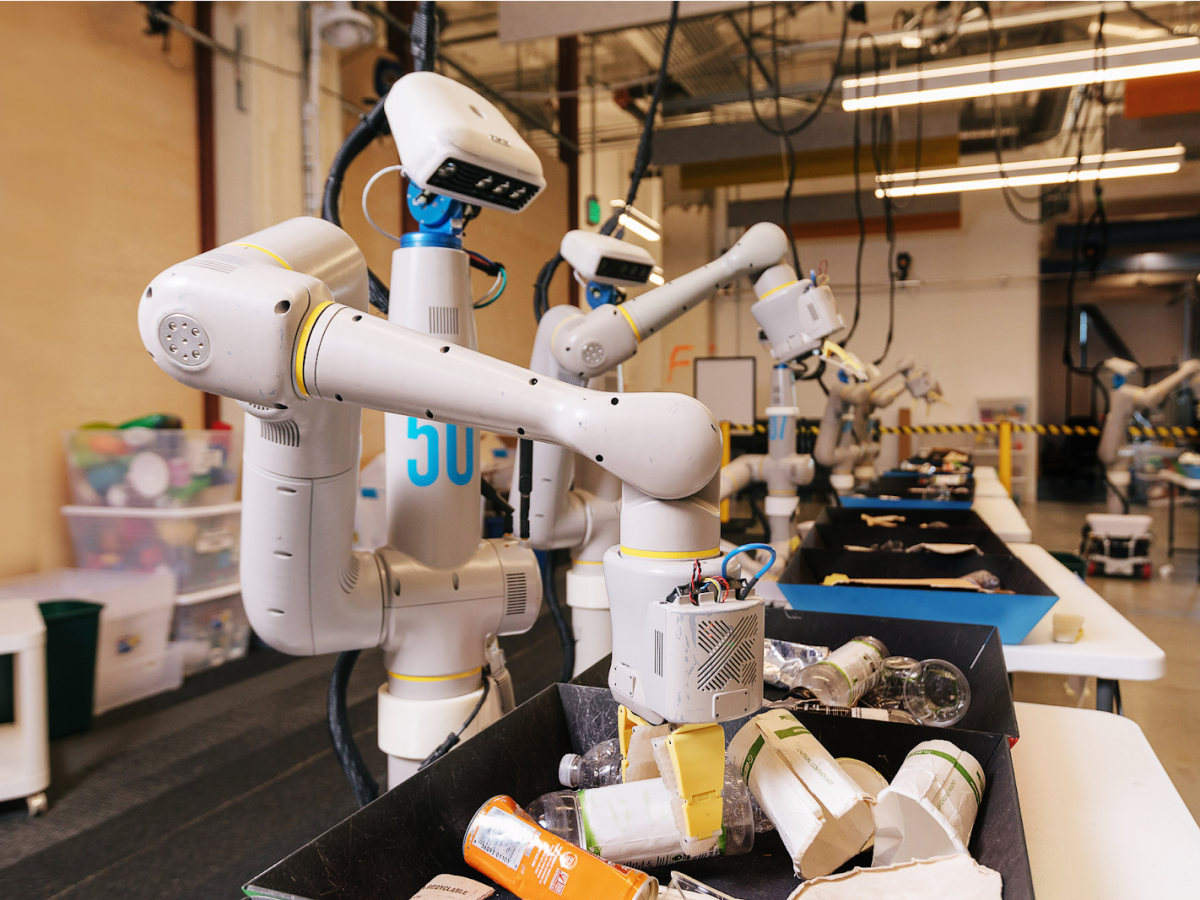
\includegraphics[width=0.8\linewidth]{Presentation/images/garbage_sorting.png}

\end{columns} 
\end{frame}

\begin{frame}
    \setlength{\leftmargini}{0cm}
    \frametitle{Цель работы:}
     Развитие методов машинного обучения с подкреплением для решения задач управления робототехническими устройствами и виртуальными агентами.

    \vspace{20pt}
    В данный момент область применения методов RL ограничена:
    \begin{itemize}
        \item[] \textbf{Вызов 1.} Sim2Real gap, при переносе агента, обученного в симуляции, на физическую установку.
        \item[] \textbf{Вызов 2.} Сложности с моделированием стратегии $\pi$, которая использует действия различной амплитуды.
        \item[] \textbf{Вызов 3.} Сходимость стратегии к локальному  оптимуму при не оптимальной функции награды.
       \item[] \textbf{Вызов 4.} Сложности с объединением RL и классических алгоритмов в рамках иерархического агента.
    \end{itemize}
\end{frame}

\iffalse
\begin{frame}
    \frametitle{Положения, выносимые на защиту}
    \begin{itemize}
        \item Метод обучения с подкреплением способный оперировать действиями различного масштаба, устойчивый к шумам, и его применение для настройки оптического интерферометра.
        \item Программно-аппаратный комплекс автоматической настройки оптического интерферометра.
        \item Метод обучения стратегии для управления движением шагающего робота с заданной линейной и угловой скоростью.
        \item Иерархический алгоритм комбинирующий алгоритмический и нейросетевой подходы и его применение для управления агентом в среде NetHack.
    \end{itemize}
\end{frame}
\note{
    Проговариваются вслух положения, выносимые на защиту
}
\fi


\begin{frame}
    \frametitle{Структура диссертационной работы}
    \begin{itemize}
        \item \underline{Глава 1.} Обзор методов обучения с подкреплением и их применения в роботике. 
        \item \underline{Глава 2.} Разработка метода, способного оперировать действиями различного масштаба, устойчивого к шумам, и его применение для настройки оптического интерферометра (вызов 1,2).
        \item \underline{Глава 3.} Метод, который позволяет достичь сходимости к хорошему оптимуму для многозадачного агента и его применение  для управления движением шагающего робота (вызов 3).
        \item \underline{Глава 4.} Иерархический алгоритм, комбинирующий алгоритмический и нейросетевой подходы и его применение для управления агентом в среде NetHack (вызов 4).
    \end{itemize}
\end{frame}

